Angle of arrival or Direction of arrival can be used to estimate the location of a prover. The signal directions are considered as straight lines and the intersection of the several pairs of these lines indicate the location of the prover. AoA is detected with the help of i) using omni directional antennas ii) multiple static antenna arrays iii) Beamforming techniques. 
\begin{figure}[htp]
    \centering
    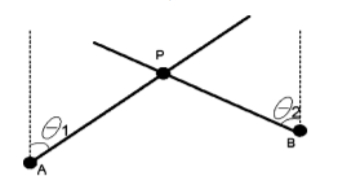
\includegraphics[width=4cm]{AoA.png}
    \caption{Angle of Arival \cite{angulation}}
    \label{fig:AoA}
\end{figure}
Once AoA is known Triangulation method can be used to find the location of the prover. Triangulation is a trigonometric approach where an unknown location is estimated based on two angles and distance between provers and verifiers. There are many limitations for location estimation based on AoA as discussed in next section. The major one is the presence of obstacles between prover and receiver. Many AoA based algorithms assume that there is a Line of Sight (LoS) between the nodes, which cannot be true in real world applications. So, there are algorithms which use help of other techniques along with AoA to do this. One of them is done using antenna arrays with array geometry and measuring differences in signal arrival times. Another method uses antenna arrays and RSSI ratios at each antenna to estimate AoA. Beamforming techniques are also used to shape the radiation pattern. 
A verification system verifies the calculated AoA with our estimated Angle. If these doesn’t match, then it means there is an attack. One advantage is that in general AoA is hard to forge by a single attacker so a distributed and a synchronized attack is required.

\begin{figure}[htp]
    \centering
    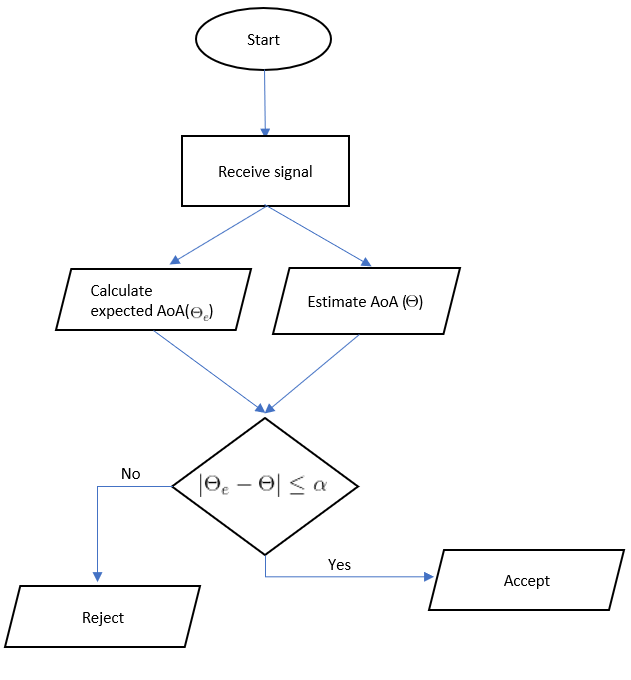
\includegraphics[width=7cm]{aoa_flow.png}
    \caption{Flow chart of a AoA based verification system \cite{abdelaziz19}}
    \label{fig:aoa_flow}
\end{figure}

As mentioned AoA based location techniques have limitations. The first and foremost being hardware dependencies i.e. for AoA to be directly measured extra hardware must be installed. Accuracy will also decrease as the distance increases between nodes. Another major drawback is that location estimation using AoA are susceptible to indoor multipath effects such as reflections, scattering, diffraction, refraction and absorption, especially in Non-Line of Sight (NLOS) conditions when shadowing occurs, this makes using these techniques in indoor conditions ineffective as it leads to erroneous measurements. A technique called fingerprinting is used to deal with multipath propagation situations. This method consists of two phases the offline phase and the online phase. In the offline phase a reference dataset is constructed by surveying signal characteristics at different know locations. In the online phase when the actual estimations is happening, measured data is compared with the reference dataset and estimation is achieved. But a major drawback for fingerprinting is that it is very labor intensive due to the offline phase, thus contributing to high deployment costs \cite{wielandt17}.